\documentclass[preprint,12pt,authoryear]{elsarticle}
\usepackage{amsmath,amssymb,amsthm}
\usepackage{booktabs}
\usepackage{graphicx}
\usepackage{caption}
\usepackage[hidelinks]{hyperref}
\newtheorem{observation}{Observation}
\newtheorem{corollary}{Corollary}
\theoremstyle{remark}
\newtheorem{remark}{Remark}
\newcommand{\R}{\mathbb{R}}
\newcommand{\E}{\mathbb{E}}
\journal{Neural Networks}

\begin{document}
\begin{frontmatter}
\title{The cosine ceiling: what random-projection Kenyon-cell codes can add to frozen embeddings}
\author{Hoang Phi Hai}
\ead{haihpaws@gmail.com}
\address{FPT School of Business and Technology (FSB), FPT University, Ho Chi Minh City, Vietnam}

\begin{abstract}
Fly-inspired codes (random projection, then $k$-winners-take-all) are placed on pretrained embeddings. With
rotation-invariant (e.g.\ Gaussian) weights, the joint law of the codes depends on the inputs only through their
cosine matrix, so any weight-independent readout is a garbling of that matrix and, on average over weights,
cannot beat the likelihood-ratio test on cosines. We give the code-overlap curve in closed form and illustrate
the bound on CelebA face embeddings. Sparse binary projections, not covered by the bound, perform here like
their rotated, covered counterparts and add nothing. Any gain over cosine must come from learned weights or a
readout's learning rule and memory budget, not from the representation.
\end{abstract}

\begin{keyword}
Kenyon cells \sep random projection \sep winner-take-all \sep locality-sensitive hashing \sep
Neyman--Pearson \sep face embeddings
\end{keyword}
\end{frontmatter}

%% ---------------------------------------------------------------------------------------------------------
\section{Introduction}
In the insect mushroom body, a few hundred projection neurons connect randomly and sparsely to thousands of
Kenyon cells (KCs), and lateral inhibition keeps only a few percent of KCs active \citep{caron2013}. \citet{dasgupta2017} read this circuit as a locality-sensitive hash: expand with a random matrix $W$,
then keep the top $k$ coordinates ($k$-winners-take-all, $k$-WTA). The ``fly hash'' and its relatives are now
applied on top of frozen pretrained features, for similarity search \citep{sharma2018,ryali2020}, word
embeddings \citep{liang2021} and continual learning with random projections \citep{mcdonnell2023}.
A practical question then arises for anyone who already has a good embedding: \emph{can a random KC layer
make inputs more discriminable than the embedding's own cosine similarity?}

Two lines of evidence point in opposite directions. Theory of random expansion shows that it amplifies noise
rather than creating separation \citep{babadi2014}, yet sparse connectivity of 5--7 inputs per KC maximises the
dimension of the representation \citep{litwinkumar2017}, which suggests that sparse wiring could matter.
Empirically, a recent connectome test found that real-valued Gaussian projections beat the fly hash on every
dataset tested and that real wiring is no better than random wiring \citep{senge2026}; design choices of
sparse randomized embeddings change search quality considerably \citep{kleyko2024}. What is missing is a
statement of what the KC layer \emph{cannot} do.

This Letter gives such a statement and illustrates it. Section~\ref{sec:theory} notes that, for rotation-invariant
$W$ such as Gaussian $W$, the joint law of the codes depends only on the cosine matrix of the inputs; it follows
that every readout of the codes that does not itself depend on $W$, however nonlinear, is bounded by the
likelihood-ratio (LR) test on cosines. We also write the expected code overlap in closed form.
Section~\ref{sec:exp} illustrates the bound on face embeddings, where the question matters for face-identifying
agents, and examines sparse binary $W$, which the theory covers only after a random rotation.
Section~\ref{sec:disc} reconciles the results with the dimension argument and lists what remains open.

%% ---------------------------------------------------------------------------------------------------------
\section{A ceiling for Gaussian projections}\label{sec:theory}
An embedding $x\in\R^d\setminus\{0\}$ is mapped to $h(x)\in\{0,1\}^m$, the indicator of the $k$ largest
coordinates of $Wx$ ($1\le k<m$). For inputs $x_1,\dots,x_n$ let $C_{ij}=\cos(x_i,x_j)$.

\begin{observation}\label{obs:1}
Let $W$ be independent of the inputs, with $WQ\overset{d}{=}W$ for every orthogonal $Q$ (e.g.\ i.i.d.\
$\mathcal N(0,1)$ entries, or $W_0Q$ with $W_0$ fixed and $Q$ Haar-distributed and independent of the inputs),
and let ties in $k$-WTA be broken by a fixed rule that depends only on the vector $Wx$ (e.g.\ lowest index).
Then the joint law of $(h(x_1),\dots,h(x_n))$ depends on the inputs only through $C$.
\end{observation}
\begin{proof}
$k$-WTA is invariant to positive scaling, so take $u_i=x_i/\|x_i\|$ and $U=[u_1,\dots,u_n]$. If
$U'^{\top}U'=U^\top U$, the map $u_i\mapsto u'_i$ is an isometry between the spans and extends to an orthogonal
$Q$ with $U'=QU$; hence $WU'=(WQ)U\overset{d}{=}WU$. The codes are a measurable function of $WU$. (For Gaussian
$W$, the rows of $WU$ are i.i.d.\ $\mathcal N(0,C)$ and ties have probability zero.)
\end{proof}

The fact is elementary: it is the invariance behind SimHash \citep{charikar2002} and rank-order hashing of
Gaussian projections \citep{eshghi2008}, the top-1 relative of
$k$-WTA; an asymptotic overlap law for a $k$-cap is known for sparse binary inputs \citep{papadimitriou2019}.
The step below is the classical reduction of a test to a maximal invariant \citep{lehmann2022}; we have not
found it stated for $k$-WTA codes.

\paragraph{Discrimination task} $K$ images $e_1,\dots,e_K$ of a person are enrolled; a query $q$ is either a new
image of that person ($Y=1$) or an image of a stranger ($Y=0$). A \emph{KC-based score} is
$S=F(h(q),h(e_1),\dots,h(e_K),Z)$ with $F$ measurable (it may include saturating plasticity, forgetting or
thresholds on the enrolled codes) and side information $Z$; neither $F$ nor the law of $Z$ may depend on $W$.
Let $C$ be the cosine matrix of $(q,e_1,\dots,e_K)$. Probabilities are per trial, over $W$, the images and $Z$.

\begin{corollary}\label{cor:1}
Let $W$ be as in Observation~\ref{obs:1} and independent of the images and $Y$, and let $Z$ be independent of
$W$, the images and $Y$. Then $S\perp Y\mid C$. Hence at every false-positive rate $\alpha$,
$\mathrm{TPR}_S(\alpha)\le\mathrm{TPR}^{*}_C(\alpha)$, where both sides allow randomisation at the threshold and
$\mathrm{TPR}^{*}_C$ is the ROC of the Neyman--Pearson test on $\Lambda=dP(C\mid Y{=}1)/dP(C\mid Y{=}0)$; in
particular $\mathrm{AUC}(S)\le\mathrm{AUC}^{*}_C$, with ties counted as $1/2$.
\end{corollary}
\begin{proof}
By Observation~\ref{obs:1}, $\Pr[S\in A\mid\text{images},Y]=K(A\mid C)$ for a Markov kernel $K$, hence
$\Pr[S\in A\mid C,Y]=K(A\mid C)$: $S$ is a garbling of $C$ \citep{blackwell1953}. A threshold test on $S$,
$\phi=\Pr[S>\tau\mid C]+\gamma\Pr[S=\tau\mid C]$, is therefore a randomised test on $C$, and by the
Neyman--Pearson lemma \citep{neyman1933} none has more power at level $\alpha$ than the test on $\Lambda$.
Integrating the ROC gives the AUC statement.
\end{proof}

\begin{remark}[the ceiling is the LR test, not raw cosine]\label{rem:lr}
Ranking by raw $T=\max_j\cos(q,e_j)$ attains the ceiling iff $\Lambda(C)$ is a.s.\ a non-decreasing function of
$T$. If negatives are selected by the very similarity being evaluated, the LR can be non-monotone, and a noisy
garbling of cosine can beat raw cosine without violating Corollary~\ref{cor:1} (Section~\ref{sec:exp}). If $Z$
depends on the images or labels but not on $W$, with $W\perp(\text{images},Y,Z)$, the ceiling is the LR test on
$(C,Z)$.
\end{remark}

\begin{remark}[one $W$ for all queries]\label{rem:onew}
A deployed system uses one $W$. Each trial's marginal law is unchanged, so the \emph{expected} operating point
over $W$ at any fixed threshold lies on or below $\mathrm{TPR}^*_C$. The AUC of a single draw, however, compares
two queries scored with the same $W$; its expectation is not the AUC bounded above. We therefore report the
\emph{cross-draw} AUC, which compares a positive and a negative scored with different, independent draws; given
the trials it is unbiased for the AUC with an independent $W$ per trial (for the population AUC, up to the
$O(1/n_{\mathrm{id}})$ weight of pairs from the same identity).
\end{remark}

\begin{remark}[trained readouts]\label{rem:trained}
The bound does not cover readouts that depend on $W$, e.g.\ trained on labelled codes made with the same $W$:
for fixed $W$ the code carries more than cosines. In $d=2$, positives at angle $+\theta$ and negatives at
$-\theta$ from $e$ have the same cosine, so $\mathrm{AUC}^*_C=1/2$, yet a readout trained on a few labelled codes
separates them. This is a fixed-$W$ statement; averaged over $W$, a readout trained on its own labelled codes is
covered by Remark~\ref{rem:loop}.
\end{remark}

\begin{remark}[closed loop]\label{rem:loop}
Let images $x_1,x_2,\dots$ be chosen by an environment whose choices and feedback are functions of past actions,
the images and randomness independent of $W$, and let the agent act on $h(x_1),\dots,h(x_t)$, the feedback and
internal randomness independent of $W$. Conditional on the whole past, the law of $Wu_t$ given
$Wu_1,\dots,Wu_{t-1}$ depends only on those values and on the cosines of $x_1,\dots,x_t$ (Observation~\ref{obs:1}
applied to $W[u_1,\dots,u_t]$; for Gaussian $W$, row-wise Gaussian with mean $c^\top G^{+}v$ and variance
$1-c^\top G^{+}c$, $G^{+}$ a pseudo-inverse), as in the conditioning technique of \citet{bayati2011}. Drawing
$Wu_t$ this way reproduces the law of the whole trajectory from these cosines and the feedback. A KC agent with
rotation-invariant $W$, including one trained online, is therefore a randomised learner on the Gram matrix of
the images seen, i.e.\ on the embeddings up to one rotation; any advantage over a \emph{specific} cosine-based
learner comes from its learning rule.
\end{remark}

\paragraph{Overlap curve} By Observation~\ref{obs:1}, the expected overlap $\kappa(c)=\E|h(x)\wedge h(y)|/k$
is a function of $c=\cos(x,y)$. As $m\to\infty$ with $p=k/m$ fixed, the $k$-WTA cut-off of the standard normal
pre-activations converges to $t=\Phi^{-1}(1-p)$, so
\begin{equation}\label{eq:kappa}
\kappa(c)\to \frac{\Pr[Z_1>t,\,Z_2>t]}{p}=\frac{1-\Phi(t)-2\,T\!\big(t,\sqrt{(1-c)/(1+c)}\big)}{p},
\end{equation}
where $Z_1,Z_2$ are standard normal with correlation $c$ and $T$ is Owen's function \citep{owen1956}. This orthant form is the dense-Gaussian case of the overlap analysis
of \citet{babadi2014}; $\kappa$ increases strictly on $[-1,1]$, with $\kappa(0)=p$ and $\kappa(1)=1$, so an overlap score is a noisy
monotone transform of cosine. It should not be used for very sparse codes ($k$ fixed, $m\to\infty$). It is the
kernel a matched non-KC baseline should use.

\paragraph{Sparse binary $W$} The thesis-style and fly-hash designs use rows with 6--10 ones
\citep{dasgupta2017,caron2013}. Such $W$ is not rotation invariant: a row with $n$ ones has
$\E[w^\top u]=(n/d)\,\mathbf 1^\top u$, so codes may also depend on each input's component along $\mathbf 1$ and
on the backbone's coordinate basis \citep{sharma2018}. Rotating the embeddings by a fresh Haar $Q$ makes the
design $W_0Q$ covered by Observation~\ref{obs:1}; comparing sparse $W$ with and without rotation therefore tests
whether the coordinate basis carries extra information.

%% ---------------------------------------------------------------------------------------------------------
\section{Experiments on face embeddings}\label{sec:exp}
\paragraph{Data} CelebA \citep{liu2015}: 182,152 images of the 7,417 identities with at least 15 images, split by
identity into tuning, test (2,966 identities) and a disjoint stranger pool. Embeddings: facenet
InceptionResnetV1 trained on VGGFace2 \citep{schroff2015,cao2018} (512-d) and DINOv2 ViT-S/14 \citep{oquab2023}
(384-d), $\ell_2$-normalised. Per test identity, $K=5$ enrolled images, 5 positive queries, 5
\emph{look-alike} strangers and 5 random strangers. To avoid selecting negatives by the score under test,
look-alikes are chosen with the \emph{other} backbone: pool identities are ranked by the cosine between the
person's enrolled prototype and a prototype built from half of their images, and the query is an unused image
from the other half (no image serves two identities). KC layer: $m=2000$, $k=100$ (5\%), score
$=\max_j |h(q)\wedge h(e_j)|$. AUC is positives versus look-alikes (29,660 trials per backbone), ties counted as
1/2; 10 draws of $W$ (and of $Q$ for rotated runs); KC AUCs are cross-draw (Remark~\ref{rem:onew}); 95\% CIs by
bootstrap over identities with the draws fixed.

\paragraph{Overlap curve and rotation} With a fresh Gaussian $W$ per pair (200 pairs per cosine), Eq.~\eqref{eq:kappa}
agrees with the Monte-Carlo mean within Monte-Carlo error (largest gap 0.0052, SE $\approx0.003$) at all 22
cosines in $[0,0.99]$ (Fig.~\ref{fig:1}a). On real pairs (600 same-person and 600 stranger pairs per backbone,
half scored after a random rotation), two-sample Kolmogorov--Smirnov tests on the independent halves do not
distinguish overlaps with and without rotation ($p\ge0.21$ for both $W$). Gaussian-$W$ overlaps match
Eq.~\eqref{eq:kappa} (mean residual $\le0.002$, within 1.1 SE); sparse-$W$ overlaps lie slightly above it
($+0.002$ to $+0.005$, 2--3 SE). These pairwise tests have limited power and do not test the joint law. On
synthetic vectors with a large common mean the same sparse $W$ fails both tests ($p$ down to $10^{-77}$); the
face embeddings spread energy over many coordinates and have little component along $\mathbf 1$ (cosine with
$\mathbf 1$ within $[-0.08,0.07]$ for 90\% of images on either backbone), as the central-limit argument for sparse projections
requires \citep{li2006}.

\paragraph{Discrimination} Table~\ref{tab:auc} gives the results. The share of positives rises monotonically
across deciles of max-cosine on both backbones, and the cross-fitted LR on that score does not exceed raw
cosine; a cross-fitted score on several entries of $C$ does, so the ceiling lies above raw cosine. All KC codes
stay below raw cosine, with CIs of the difference excluding zero. Sparse codes without rotation equal the
covered, rotated design within draw-to-draw variation (per-draw SD $\le0.005$); the upper 95\% limits of sparse
minus raw cosine are $-0.0014$ (facenet) and $-0.008$ (DINOv2), so a sparse gain is excluded. Projecting every
embedding off $\mathbf 1$ leaves sparse minus raw cosine at $-0.0017$ and $-0.0115$.

\begin{table}[p]\centering
\caption{AUC, same person versus look-alike stranger (look-alikes selected with the other backbone, so the
columns are different tasks). KC rows: cross-draw AUC over 10 draws; ``rot.'' = embeddings randomly rotated
first, which makes sparse $W$ a covered design. Brackets: 95\% CI, bootstrap over identities.}\label{tab:auc}
\footnotesize\setlength{\tabcolsep}{4pt}
\begin{tabular}{lcc}\toprule
 & facenet & DINOv2\\\midrule
score on $C$, cross-fitted (ceiling $\ge$) & 0.992 & 0.705\\
LR on max-cosine, cross-fitted & 0.986 & 0.683\\
raw cosine & 0.987 [.986, .989] & 0.685 [.678, .691]\\
KC Gaussian $W$ (no rot.\ / rot.) & 0.986 / 0.986 & 0.674 / 0.676\\
KC sparse $W$ (no rot.\ / rot.) & 0.986 / 0.986 & 0.673 / 0.676\\
sparse $-$ cosine, no rot. & $-.0016$ [$-.0019$, $-.0015$] & $-.0115$ [$-.0127$, $-.0102$]\\
sparse $-$ cosine, rot. & $-.0016$ [$-.0018$, $-.0014$] & $-.0092$ [$-.0102$, $-.0080$]\\
Gaussian $-$ cosine, no rot. & $-.0014$ [$-.0016$, $-.0012$] & $-.0104$ [$-.0114$, $-.0094$]\\
\bottomrule\end{tabular}

\vspace{1.5em}
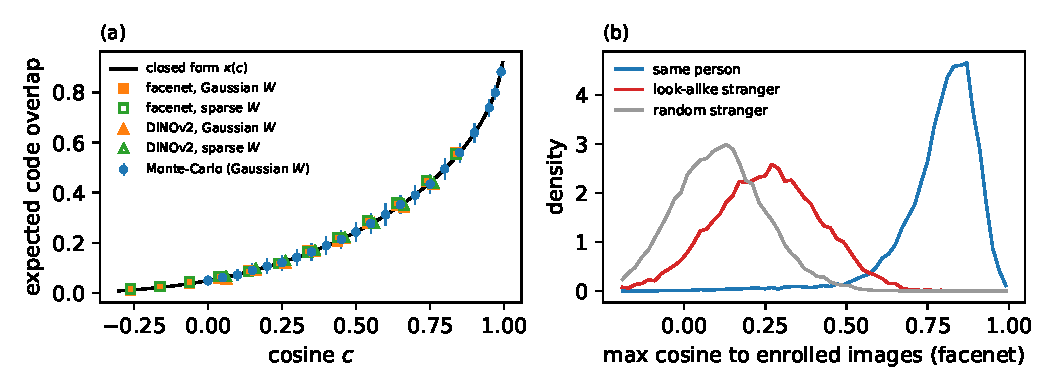
\includegraphics[width=\textwidth]{fig1.pdf}
\captionsetup{type=figure}
\caption{(a) Expected KC code overlap: closed form Eq.~\eqref{eq:kappa} (line), Monte-Carlo with Gaussian $W$
(dots, $\pm$SD), and real face pairs for Gaussian and sparse binary $W$, as means of per-pair overlaps in cosine
bins of width 0.1 (open markers; squares facenet, triangles DINOv2). (b) Max cosine of a query to the enrolled
images on facenet, with look-alikes selected with DINOv2: they sit between random strangers and the same person.}\label{fig:1}
\end{table}

\paragraph{A selection artefact} In a first version of the task, look-alikes were the pool \emph{images} most
similar to the prototype in the evaluated embedding. For DINOv2 this inverts the LR: in one run, raw cosine
scores an AUC of 0.220, below chance, and Gaussian KC codes score 0.229 (cross-draw) --- apparently above the
``ceiling''. It is not a violation: the cross-fitted LR on the same statistic, itself a lower bound on the
ceiling, is 0.784 (Remark~\ref{rem:lr}). Even identity-level selection in the evaluated embedding left a mild
non-monotone LR on facenet, which is why the main task selects with the other backbone. The lesson is general
for evaluations of bio-inspired codes: state the ceiling as the LR test, and never select negatives by the
score under test.

%% ---------------------------------------------------------------------------------------------------------
\section{Discussion}\label{sec:disc}
\paragraph{Relation to the dimension argument} \citet{litwinkumar2017} show that sparse
connectivity maximises the dimension of KC representations of low-dimensional, noisy inputs, which helps a
\emph{linear} readout learn many associations. Corollary~\ref{cor:1} is about a different quantity: the best
achievable discrimination by any readout that does not depend on $W$. Both can hold. A KC code may make a
simple, trained readout learn faster, but for a fixed comparison it does not raise the ceiling of a learner that
has the cosines and the same labels (Remarks~\ref{rem:trained}--\ref{rem:loop}). On dense, normalised embeddings
of several hundred dimensions, our data also suggest that 6--10-input sums already behave like Gaussian
projections \citep{li2006}, so the distinction between sparse and dense wiring largely disappears.

\paragraph{The connectome result} \citet{senge2026} found that real-valued Gaussian projections beat the fly
hash and that connectome wiring adds nothing over random wiring. Corollary~\ref{cor:1} is consistent with this
but does not explain it: fly-hash and connectome $W$ are not rotation invariant, and the bound does not order
two codes below it. For the same $W$, binarisation is a further garbling, and our results suggest that on dense
embeddings fixed sparse wiring behaves like a covered design. Learned projections such as BioHash
\citep{ryali2020} and FlyVec \citep{liang2021} escape the bound because $W$ depends on the data; readouts trained
on rotation-invariant codes, as in expand-and-sparsify expressivity results \citep{dasgupta2020}, remain
randomised learners on cosines (Remark~\ref{rem:loop}).

\paragraph{Implications} For systems that put a fly-inspired layer on frozen features, a random KC layer
should be expected to preserve, not improve, discriminability, and a kernel baseline using Eq.~\eqref{eq:kappa}
isolates the effect of the representation from that of the readout. Any remaining advantage over a given cosine
baseline comes from learned weights or from the readout's learning rule, and any other benefit is in resources,
e.g.\ fixed-size familiarity signals that store no exemplars, not in the ceiling.

\paragraph{Limitations} The bound concerns expected operating points and the cross-draw AUC over $W$; a single
fixed $W$, and in particular its own AUC, is not covered, although for large $m$ each overlap concentrates around
$\kappa(\cos)$. The sparse-$W$ result without rotation is empirical, on one dataset and two backbones; embeddings with energy
concentrated in few coordinates may behave differently \citep{kleyko2024}. Our ceiling estimates are cross-fitted
functions of $C$ and therefore lower bounds on the true ceiling. Look-alikes are selected with the other
backbone, so the two columns of Table~\ref{tab:auc} are different tasks.

\section*{Data and code availability}
Code, summary results and a seeded script that rebuilds the identity-disjoint splits from the original CelebA
files are available at \url{https://github.com/haihpse150218/kc-cosine-ceiling} and archived on Zenodo
\citep{hoang2026code}. CelebA images, identity labels and per-image
embeddings are not redistributed, as the CelebA agreement does not permit it.

\section*{Declaration of generative AI and AI-assisted technologies in the manuscript preparation process}
During the preparation of this work the author used Claude (Anthropic), through the Claude Code
assistant, in order to help write the simulation and analysis code, search the literature, check reference
metadata against Crossref and arXiv, and draft and edit the text. After using this tool, the author reviewed
and edited the content as needed and takes full responsibility for the content of the published article.

\bibliographystyle{elsarticle-harv}
\bibliography{refs}
\end{document}
